
\documentclass[tikz,border=2pt]{standalone}
\usepackage{amsmath,amssymb}
\usepackage{amsfonts}
\usepackage{xcolor}
\usetikzlibrary{arrows.meta,positioning,calc,shapes,decorations.pathreplacing}
% Define some common colors used in IR lectures if any
\definecolor{sparse}{rgb}{0.8,0.8,1}
\definecolor{dense}{rgb}{1,0.8,0.8}
\begin{document}
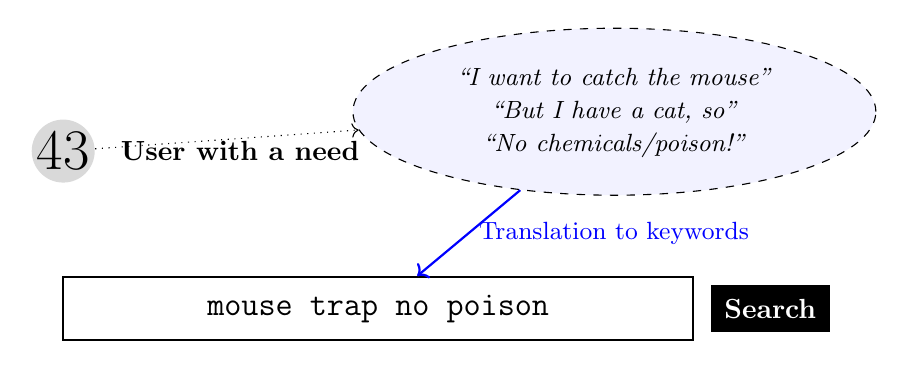
\begin{tikzpicture}[
    searchbox/.style={rectangle, draw, thick, minimum width=8cm, minimum height=0.8cm, font=\large},
    user/.style={circle, fill=gray!30, minimum size=0.8cm},
    icon/.style={font=\huge}
]
    
    \node[user] (u) at (0,3) {};
    \node[icon] at (u) {\ding{43}}; 
    \node[right=0.2cm of u] {\textbf{User with a need}};

    
    \node[searchbox, fill=white] (box) at (4,1) {\texttt{mouse trap no poison}};
    \node[right=0.2cm of box, fill=black, text=white, inner sep=5pt] {\textbf{Search}};
    
    
    \node[draw, ellipse, dashed, fill=blue!5, minimum width=4cm, minimum height=1.5cm] (intent) at (7,3.5) {
        \begin{tabular}{c}
            \small \textit{``I want to catch the mouse''} \\
            \small \textit{``But I have a cat, so''} \\
            \small \textit{``No chemicals/poison!''}
        \end{tabular}
    };
    \draw[->, dotted] (u) -- (intent);
    \draw[->, thick, blue] (intent) -- (box) node[midway, right] {\small Translation to keywords};
\end{tikzpicture}
\end{document}
